\documentclass{book}

\usepackage{graphicx}
\usepackage{listings}
\usepackage[ngerman]{babel}

\begin{document}

\tableofcontents

\newpage

% ==================== Installation ====================
\setcounter{chapter}{1}

\section{Installation}

Um das Programm zu installieren, benötigen sie zunächst sowohl eine valide JDK installation, als auch eine Gradle installation. Wenn sie eine der beiden nicht haben, verfolgen sie bitte folgenden zwei Installationsanleitungen. Sollten sie sowohl eine JDK als auch eine Gradle Installation schon haben, so können sie bei Punkt 0.0.3 weiterlesen.

% ==================== JDK INSTALLATION ====================
\subsection{JDK Installation}

Sie benötigen zunächst eine valide JDK Installation. JDK steht für Java Development Kit und wird verwendet um Java Programme zu entwickeln.
Bei unserem Programm können sie eine beliebige JDK mit einer Version von 8+ herunterladen. Wir werden die Vorgehensweise einer Installation von JDK  8 als Beispiel durchführen.

% ==================== WINDOWS ====================
\subsubsection{Windows JDK Installation}

Navigieren sie bitte auf die Webseite https://www.ninite.com . Ninite ist eine Webseite mit welcher man mehrere Programme gleichzeitig automatisiert herunterladen kann. Dort werden sie unter ''Developer Tools'' eine JDK Version mit dem Namen ''JDK (AdoptOpenJDK) x64 8'' sehen. Kreuzen sie die box daneben mit einem Mausclick an. Scrollen sie nun ganz herunter und clicken sie auf den Knopt ''Get Your Ninite''. Führen sie die heruntergeladene Datei aus, welche dann automatisch JDK 8 installieren wird.

\begin{figure}[h!]
\centering
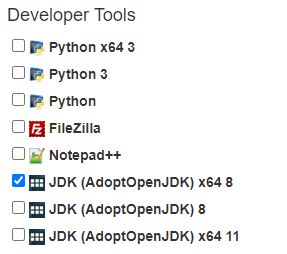
\includegraphics[width=0.5\linewidth]{Windows.JPG}
\end{figure}

Um zu verifizieren das JDK korrekt installiert wurde, öffnen sie ein CMD oder Powershell Fenster, entweder durch ihre Apps oder mit Strg + R, tippen sie dann CMD oder Powershell und drücken sie Enter. Geben sie im geöffneten Fenster das Kommando Javac ein und drücken sie Enter. Sollte nichts passieren, und sie einen Fehler bekommen, so wurde das JDK nicht korrekt installiert und sie müssen das folgende Subkapitel auch noch durchgehen. Wird das Kommando wie im Bild korrekt ausgeführt, so können sie beim Kapitel ''Gradle Installation'' weiterlesen. 

\begin{figure}[h!]
\centering
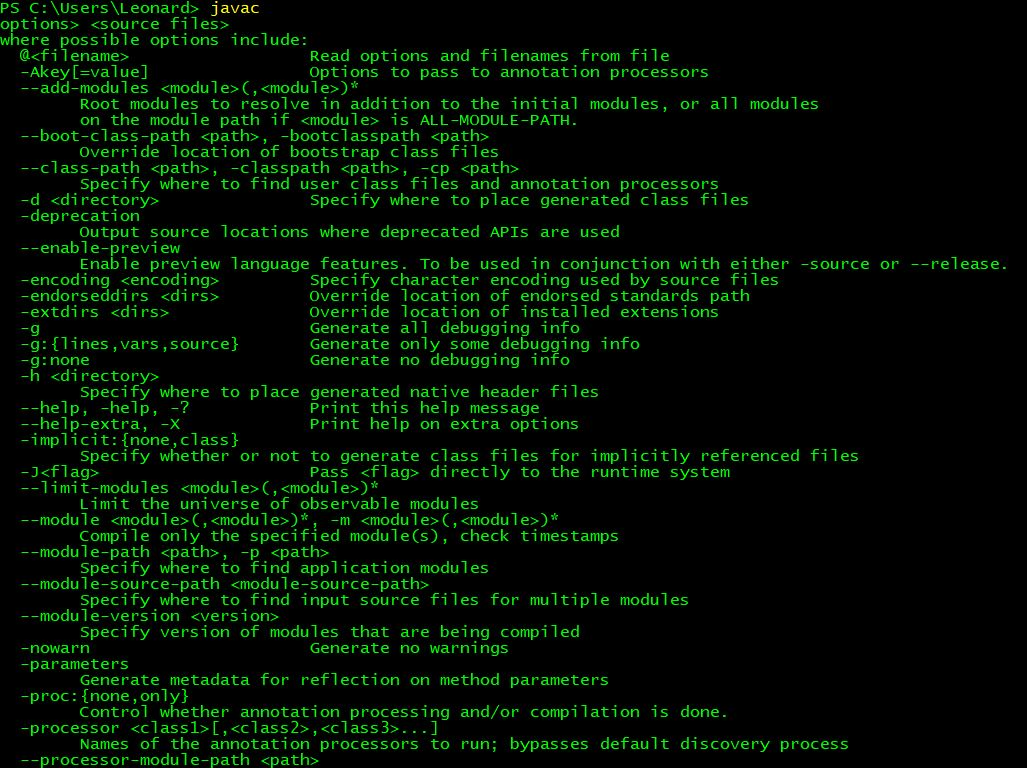
\includegraphics[width=\linewidth]{JavacWindows.JPG}
\end{figure}


\newpage
\paragraph{PATH und JAVA\textunderscore HOME}

Sollte das Kommando im letzten Schritt ein Fehler angezeigt haben, so ist JDK nicht korrekt konfiguriert. Um dieses zu ändern, navigieren sie bitte zu dem Installationspfad ihrer Jdk, welcher einen Namen wie ''C:/Program Files/Java/jdk-version haben wird''. In diesem Ordner werden sie einen weiteren Ordner ''bin'' finden und erst einmal öffnen. Kopieren sie nun den Pfad dieses Ordners (z.B. ''C:/Program Files/Java/jdk-12.0.2/bin'' für JDK 12.0.2) und öffnen sie unter Windows XP/7 My PC, oder unter Windows 8+/10 This PC. Clicken sie die rechte Maustaste und wählen sie ''Properties'' aus.
\begin{figure}[h!]
\centering
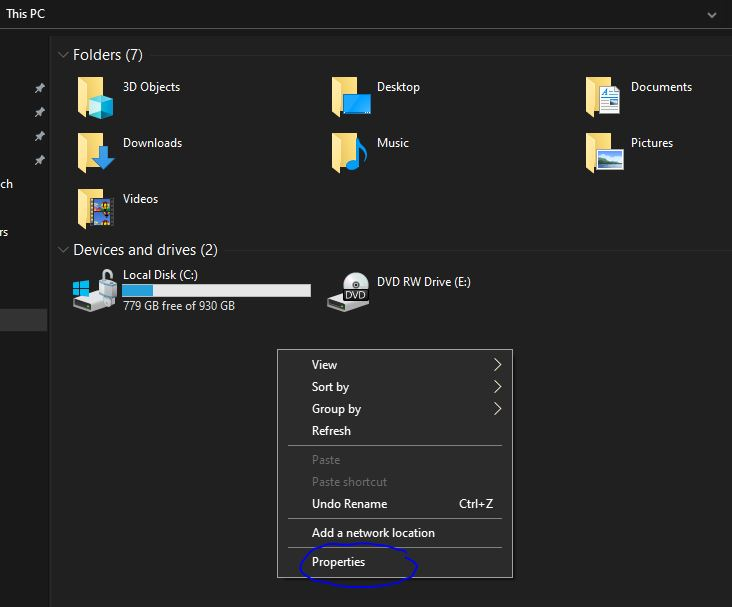
\includegraphics[width=0.7\linewidth]{Properties.JPG}
\end{figure}

In dem geöffneten Fenster auf der linken Seite werden sie einen Knopf ''Advanced System Settings'' sehen, welchen sie nun anclicken.
\begin{figure}[h!]
\centering
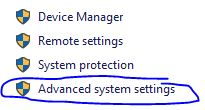
\includegraphics[width=0.5\linewidth]{AdvancedSystemSettings.JPG}
\end{figure}

\newpage
In dem nun geöffneten Fenster, ganz unten Rechts, clicken sie auf den Knopf ''Environment Variables''.
\begin{figure}[h!]
\centering
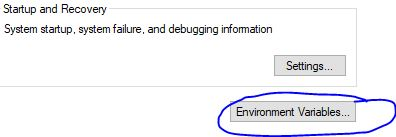
\includegraphics[width=0.5\linewidth]{EnvironmentVariables.JPG}
\end{figure}

Hier sind alle Variablen von Programmen die Windows durch die Konsole erkennt vorhanden. Wr müssen nun unsere JDK Installation dazufügen. Um dieses zu tun, clicken sie bei den ''System Variables'' auf den ''New...'' Knopf und geben der Variable den Namen ''JAVA\textunderscore HOME'', beachten sie das der Name korrekt und groß geschrieben ist, und als Pfad geben sie den kopierten Pfad ohne die ''/bin'' endung an, also z.B. '''C:/Program Files/Java/jdk-12.0.2'' und clicken sie dann auf Ok.
\begin{figure}[h!]
\centering
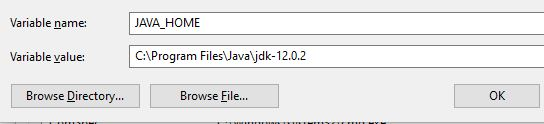
\includegraphics[width=\linewidth]{JAVA_HOME.JPG}
\end{figure} 

\textbf{(*)}
Jetzt müssen sie nur noch ihre System PATH Variable bearbeiten um Java als System Variable einzufügen. Um dieses zu tun, scrollen sie unter ''System Variables'' runter bis sie eine Variable mit dem Namen ''Path'' sehen, und dann diese doppelclicken. In dem jetzt angezeigtem Fenster sind sämtliche Programme die von Windows als System Variablen erkannt werden drin. Clicken sie rechts auf ''New'' und fügen sie den gesamten kopierten Pfad ein und drücken sie Enter. Sie können nun alle Fenster schließen. 
\begin{figure}[h!]
\centering
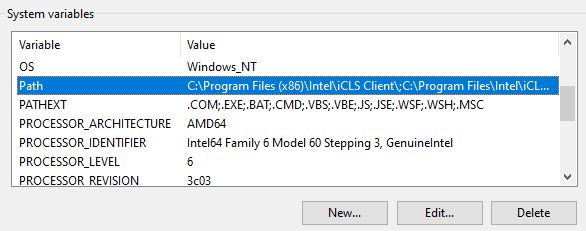
\includegraphics[width=\linewidth]{SystemVariables.JPG}
\end{figure} 

% ==================== LINUX ====================
% TODO ADD LINUX AND MACOS

% ==================== GRADLE INSTALLATION ====================
\subsection{Gradle Installation}

Nun werden wir Gradle installieren. Gradle is ein ein Tool mit welchem man Java Applikationen bauen kann.

% ==================== WINDOWS ======================
\subsubsection{Windows Gradle Installation}

Navigieren sie auf die Webseite https://gradle.org/install/ und scrollen sie runter zu ''Installing manually''. Clicken sie dort auf ''Binary-only'' welches Gradle herunterladen sollte.
\begin{figure}[h!]
\centering
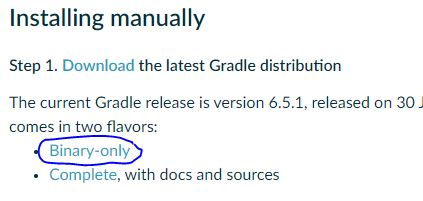
\includegraphics[width=0.5\linewidth]{GradleDownload.JPG}
\end{figure} 

Extrahieren sie die heruntergeladene ZIP datei und kopieren sie den Pfad der bin datei in der Gradle datei, z.B. ''PFAD/gradle-6.4.1/bin'' und erstellen für diesen einen neuen Eintrag in der System Path Variable, siehe (*) bei der JDK Installation. Sie sollten nun die Möglichkeit haben in einem CMD oder Powershell fenster das Kommando ''gradle -version'' ausführen zu können.

% ==================== Application Installation ==================== 

\end{document}